\documentclass[conference]{IEEEtran}
\IEEEoverridecommandlockouts
% The preceding line is only needed to identify funding in the first footnote. If that is unneeded, please comment it out.
\usepackage{cite}
\usepackage[portuges,brazil,english]{babel}
\usepackage{amsmath,amssymb,amsfonts}
\usepackage{algorithmic}
\usepackage{graphicx}
\usepackage{textcomp}
\usepackage[export]{adjustbox}
\usepackage{float}
\usepackage[ruled,vlined,linesnumbered,portuguese]{algorithm2e}
\usepackage[utf8]{inputenc}
\def\BibTeX{{\rm B\kern-.05em{\sc i\kern-.025em b}\kern-.08em
    T\kern-.1667em\lower.7ex\hbox{E}\kern-.125emX}}
\begin{document}

\title{Trabalho 3 - MC886 Aprendizado de Máquina}

\author{\IEEEauthorblockN{Leo Yuuki Omori Omi}
\IEEEauthorblockA{
138684 \\
leoyuuki@gmail.com}
\and
\IEEEauthorblockN{João Pedro Ramos Lopes}
\IEEEauthorblockA{
139546 \\
jpedrorl@gmail.com}}

\maketitle

\section{Introdução}

Neste trabalho, tivemos que agrupar vários textos utilizando utilizando técnicas de Aprendizado não-supervisionado. Utilizando dados em formato \textit{bag-of-words} utilizamos algumas técnicas para tentar achar agrupamentos que fizessem algum sentido.

\subsection{Soluções Propostas}

\subsubsection{DBSCAN}
Tentamos utilizar a técninca Density-Based Spatial Clustering of Applications with Noise (DBSCAN), já implementado na biblioteca Scikit Learn. Tentamos variar os parâmetros \textit{eps} e \textit{min\_samples}, no entanto, inicialmente, não conseguimos achar uma configuração que desse um resultado que parecia coerente, portanto desistimos de continuar experimentos com esta técnica. Possivelmente, a distribuição dos dados não favorecia o DBSCAN ou mesmo foi uma escolha infortúnia do parêmtros.

\subsubsection{Hierarchical Clustering}


\subsubsection{K-means}


\subsection{Experimentos}
\subsubsection{Modelos iniciais}
Para analisar o número de grupos presentes no problema, utilizamos como modelo base o Elbow Method, variando esse número no intervalo [10, 1000] com passo 10 encontramos o gráfico disposto na figura \ref{fig:elbow}. 

\begin{figure}[H]
  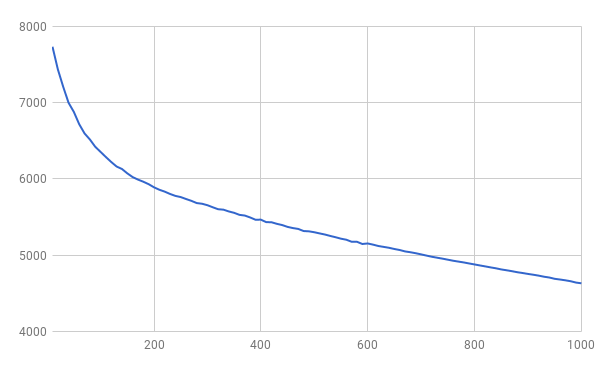
\includegraphics[scale=0.4, center]{elbow.png}
  \caption{Número de Clusters x Erro médio}
  \label{fig:elbow}
\end{figure}

Utilizando o modelo de k-médias com 3 reinícios, 10 iterações e inicialização aleatória \textit{k-means++}. Com base no gráfico gerado, escolhemos o range de classes [50, 400] a ser submetido ao método de silhueta. Utilizando passo 50 encontramos o gráfico da figura \ref{fig:sil1}, que representa a pontuação para tais valores de k.

\begin{figure}[H]
  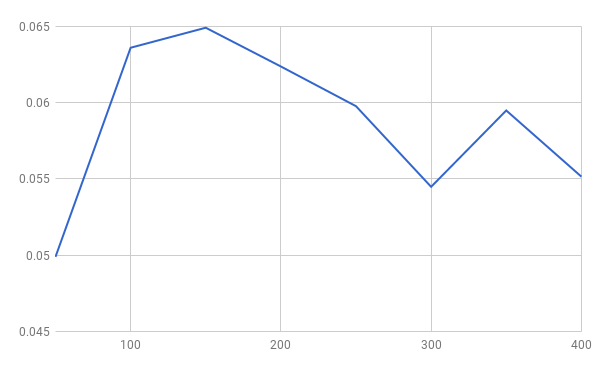
\includegraphics[scale=0.4, center]{silhouette1.png}
  \caption{Silhueta no intervalo [50, 400] com passo 50}
  \label{fig:sil1}
\end{figure}

Finalmente, para determinar o número de classes a ser utilizado pelo modelo, foi percorrido o intervalo [125, 175] e desenhado o gráfico da pontuação encontrada pelo método de silhueta, representado na figura \ref{fig:sil2}. Dessa forma, foram emscolhidas 151 clusters para o problema. 

\begin{figure}[H]
  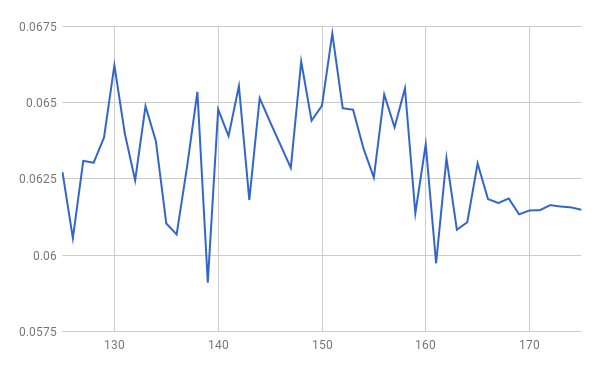
\includegraphics[scale=0.4, center]{silhouette2.png}
  \caption{Silhueta no intervalo [125, 175]}
  \label{fig:sil2}
\end{figure}


\subsubsection{Solução Base (One vs All)}
A solução base que utiliza como \textit{features} os níveis de cinza de todos os pixels da imagem obteve uma acurácia para o conjunto de testes de 35\% e para o de validação 28\%. A diferença de 7\% entre a acurárcia dos dois conjuntos indica que houve um pouco de \textit{overfitting} neste caso, e além disso, obtivemos um resultado pouco satisfatório.

\subsubsection{Solução Base Melhorada}
Com o intuito de de melhorar a solução base, foram feitos experimentos utilizando funções de borda e de segmentação. A solução de função de borda trouxe resultados na média muito próximos à solução original. Poderíamos concluir à partir deste resultado, que a extração de bordas da imagem não extrai dados que sejam relevantes para a melhora do modelo, e é algo que a própria regressão logística sobre os valores de cinza da imagem original acaba considerando de certa maneira.

\begin{figure}[H]
  
\includegraphics[center]{bor.png}
  \caption{Operador de borda}
  \label{fig:frog1}
\end{figure}

A segunda solução utilizando a segmentação obteve resultados piores de acurácia. 30\% para o conjunto de testes e 21\% no conjunto de validação. A causa desta queda pode ser atribuído à técnica simples da segmentação, já que em alguns casos a máscara pode extrair o objeto da imagem e em outros o plano de fundo, dependendo dos níveis de cinza do objeto serem maiores ou menores que o do fundo. Portanto, não obtivemos melhoras significativas com estas soluções, portanto iremos utlizar os níveis de cinza como na primeira solução proposta para as próximas soluções do trabalho.

\begin{figure}[H]
  
\includegraphics[center]{seg1.png}
  \caption{Segmentação isolando o plano de fundo}
  \label{fig:boat1}
\end{figure}

\begin{figure}[H]
  
\includegraphics[center]{seg2.png}
  \caption{Segmentação isolando o objeto}
  \label{fig:frog1}
\end{figure}

\subsubsection{Solução Base PCA}
A solução utilizando o PCA, deu resultados bons. Foi escrito um programa rodando em um laço com valores crescentes para o número de compenentes, começando com 15 componentes e aumentando em 16 em cada iteração. A execução do problema é lenta, mas nos trouxe resultados que puderam ser aproveitados. Por volta de 40 componentes, obtemos uma acurácia de 30\% tanto para o conjunto de treino como o conjunto de validação, o que foi o melhor resultado observado utilizando a regressão logística. Como obtemos uma acurácia semelhante entre os dois conjuntos, poderíamos dizer que não está ocorrendo \textit{overfitting}, diferente das soluções anteriores. Além disso, como diminuímos a dimensionalidade do modelo, obtemos uma solução computacionalmente mais leve.

\begin{table}[H]
\centering
\caption{Tabela de acurácia por número de componentes}
\label{my-label}
\begin{tabular}{lllll}
Componentes & Acurácia Treino & Acurácia Validação & & \\
15  & 0.29 & 0.29 &  &  \\
31  & 0.3  & 0.3  &  &  \\
47  & 0.3  & 0.3  &  &  \\
63  & 0.31 & 0.3  &  &  \\
79  & 0.31 & 0.3  &  &  \\
95  & 0.31 & 0.3  &  &  \\
111 & 0.31 & 0.3  &  &  \\
127 & 0.31 & 0.3  &  &  \\
143 & 0.32 & 0.3  &  &  \\
159 & 0.32 & 0.3  &  &  \\
175 & 0.32 & 0.3  &  &  \\
191 & 0.32 & 0.3  &  &  \\
207 & 0.32 & 0.3  &  &  \\
223 & 0.32 & 0.3  &  &  \\
239 & 0.32 & 0.3  &  &  \\
255 & 0.32 & 0.3  &  &  \\
271 & 0.32 & 0.29 &  &  \\
287 & 0.32 & 0.29 &  &  \\
303 & 0.32 & 0.29 &  &  \\
319 & 0.32 & 0.29 &  &  \\
335 & 0.32 & 0.29 &  &  \\
351 & 0.33 & 0.29 &  &  \\
367 & 0.33 & 0.29 &  &  \\
383 & 0.33 & 0.29 &  &  \\
399 & 0.33 & 0.29 &  &  \\
415 & 0.33 & 0.29 &  & 
\end{tabular}
\end{table}

\subsubsection{Solução Base (Multinomial)}
Para esta solução, usando a regressão multinomial com PCA, obtivemos também uma acurácia de 30\% para o conjunto de testes e 30\% para o de validação. Um resultado semelhantes ao do One vs All, não obtendo uma melhora o resultado em comparação com a solução anterior.


\section{Redes Neurais}
Redes Neurais agrupam métodos de aprendizado de máquina que foram originalmente baseados no comportamento do cérebro, onde neurônios fazem operações simples e a complexidade do sistema está na iteração entre os diversos neurônios. Apesar de os conceitos aplicados atualmente estarem distantes dos modelos cerebrais, Redes Neurais estão no Estado da Arte na solução de diversos problemas complexos. 

Uma Rede Neural é dividida em 3 camadas, cada uma composta por uma matriz de pesos e uma função de ativação: \textit{Input Layer}, \textit{Hidden Layer} e \textit{Output Layer}. A entrada é multiplicada pela primeira camada e submetida a função de ativação, onde sua saída é multiplicada pela matriz subsequente e assim por diante. 

Existem diversas operações que podem substituir a multiplicação de matrizes, como uma operação Convolucional 2D (utilizado particularmente em problemas relacionados a Visão Computacional) em que filtros são aplicados de maneira convolucional a entrada. 

\subsubsection{Soluções Propostas}
Para construir diversos modelos, consideramos os operadores \textit{Dense($X$)} que realiza a operação $output = dot(input, kernel) + bias$ utilizando $X$ neurônios; \textit{Conv2D(32, (3, 3))}, que utiliza 32 filtros de aprendizado de tamanho $3x3$. Como operador de ativação, foi considerado o operador ReLU (\textit{Rectified Linear Unit}) que aplica a operação $f(x) = max(x, 0)$. 

Na camada de entrada e de saída foram utilizados os operadores \textit{Dense(512} e \textit{Dense(10)}, respectivamente. A saída foi ligada a um operador \textit{softmax}, a fim de classificar as imagens nas 10 classes do problema. Na \textit{Hidden Layer} foram feitas as composições de operadores sequenciais a seguir, cujos resultados encontram-se nas imagens indicadas. As duas últimas se tratam de camadas compostas.

\begin{itemize}
	\item Dense(512) - Figura \ref{fig:dense}
	\item Conv2D(32, (3, 3)) - Figura \ref{fig:conv}
	\item Dense(512) \& Conv2D(32, (3, 3)) - Figura \ref{fig:dense_conv}
	\item Conv2D(32, (3, 3)) \& Dense(512) - Figura \ref{fig:conv_dense}
\end{itemize}

\begin{figure}[h!]
	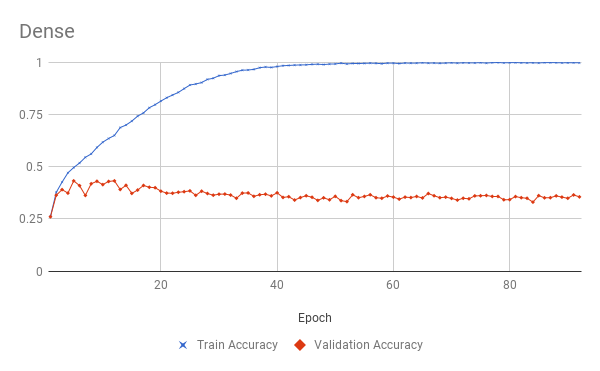
\includegraphics[scale=0.4]{dense.png}
	\caption{Acuracia para treino e validação}
	\label{fig:dense}
\end{figure}

\begin{figure}[h!]
	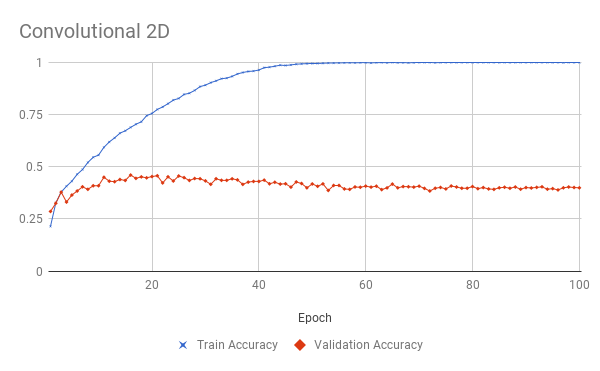
\includegraphics[scale=0.4]{conv.png}
	\caption{Acuracia para treino e validação}
	\label{fig:conv}
\end{figure}

\begin{figure}[h!]
	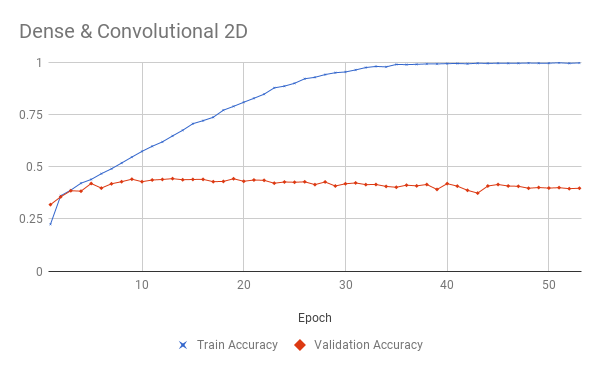
\includegraphics[scale=0.4]{dense_conv.png}
	\caption{Acuracia para treino e validação}
	\label{fig:dense_conv}
\end{figure}

\begin{figure}[h!]
	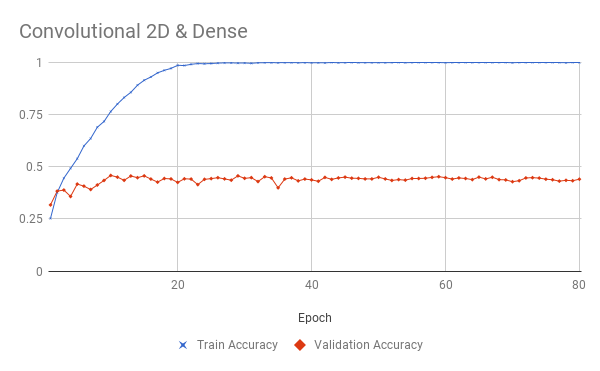
\includegraphics[scale=0.4]{conv_dense.png}
	\caption{Acuracia para treino e validação}
	\label{fig:conv_dense}
\end{figure}

Por conta da dimensão do conjunto de treino, foram utilizadas apenas 10\% das entradas. Então, o conjunto de treino foi dividido em treino e validação (utilizando uma proporção de 0.7) a fim de validar os modelos propostos. Os melhores resultados do conjunto de validação para cada modelo foram: 

\begin{itemize}
	\item Dense(512) - $0.4327$
	\item Conv2D(32, (3, 3)) - $0.4607$
	\item Dense(512) \& Conv2D(32, (3, 3)) - $0.4433$
	\item Conv2D(32, (3, 3)) \& Dense(512) - $0.4587$
\end{itemize}

Aplicando a rede neural encontrada nas melhores épocas para o modelo \textit{Conv2D(32, (3, 3))} e para o modelo \textit{Conv2D(32, (3, 3)) \& Dense(512)} utilizando o conjunto de testes, encontrou-se uma acuracia de $0.4673$ e $0.4374$, respectivamente. 

A maior acuracia encontrada pela rede \textit{Conv2D(32, (3, 3))} pode ser atribuida a quantidade reduzida de dados utilizados, visto que por ser uma rede mais simples necessita de menor número de treinos para calibrar seus valores. 

Finalmente, a fim de comparar a Ativação utilizando \textit{ReLU}, executou-se o modelo \textit{Conv2D(32, (3, 3)) \& Dense(512)} utilizando como método de ativação a Tangente Hiperbólica: $f(x) = htan(x)$. A maior acurácia encontrada para o conjunto de validação foi de $0.3320$, apontando uma vantagem para a utilização do \textit{ReLU}. 

\section{Conclusões}
Sobre as soluções propostas, aquelas que se utilizaram de processamento de imagem não trouxeram melhoras para o modelo. No entanto, a solução utilizando PCA trouxe melhoras tanto para o resultado quanto para tempo de computação do modelo, demonstrando a vantagem de usar a redução de dimensionalidade por este método.

Com relação a modelagem utilizando Redes neurais, poderia-se estudar a acuracia para um número maior de camadas, além da utilização mais estensiva de operadores convolucionais. Outra analise que pode ser feita em estudos posteriores é a utilização de Dropout, que utiliza da desativação de neurônios aleatórios de uma camada, evitando overfit e gerando redundâncias na rede neural. 

\begin{thebibliography}{00}
\bibitem{linearregression1} Montgomery, D.C., Peck, E.A. and Vining, G.G., 2015. Introduction to linear regression analysis. John Wiley \& Sons.
\bibitem{gendreau2010handbook} Gendreau, M. and Potvin, J.Y., 2010. Handbook of metaheuristics (Vol. 2). New York: Springer.
\bibitem{continousgenetics} Haupt, R.L. and Haupt, S.E., 2004. Practical genetic algorithms. John Wiley \& Sons.
\bibitem{continuousgenetics2} Djurisic, A.B., Elazar, J.M. and Rakic, A.D., 1997. Genetic algorithms for continuous optimization problems-a concept of parameter-space size adjustment. Journal of Physics A: Mathematical and General, 30(22), p.7849.
\end{thebibliography}

\end{document}
